\documentclass{article}
\usepackage{polski}
\usepackage[utf8]{inputenc}
\usepackage{listings}
\usepackage{graphicx}
\usepackage{amsmath}  % dla matematycznych symboli

\title{AiSD Lista 1}
\author{Dominik Kowalczyk}

\begin{document}
	\maketitle  
	
	\section{Algorytm sortowania INSERTION SORT (przez wstawianie)}
	
\large {W podstawowej wersji (bez modyfikacji) algorytmu sortowania przez wstawienie wyróżniamy następujący fragment kodu: }

	\begin{lstlisting}[language=C++, caption={Kod dla funkcji sortującej przez wstawienie}, numbers=left, frame=single, xleftmargin=20pt]
void INSERTION_SORT(int A[], int n) {
	for (int i = 1; i < n; i++) {
		int key = A[i];
		int j = i - 1;
		while (j >= 0 && A[j] > key) {
			A[j + 1] = A[j];
			j--;
		}
		A[j + 1] = key;
		}
	}
	\end{lstlisting}
	
\large {Powyższy fragment kodu zaczyna się od funkcji for, która przechodzi kolejno po każdym elemencie tablicy \(A\). Naszą iterację zaczynamy od drugiego elementu tablicy (z indeksem \(1\)) (zakładając, że \(0\) jest już posortowany). Zmienna \(key\) umożliwia przechowanie wartości wstawianego elementu zapobiegając  nadpisaniu oraz pozwalając na porównywanie tej wartości z kolejnymi elementami posortowanego ciągu. Gdy napotkany element w posortowanej części jest większy od wstawianego, przesuwamy go o jedną pozycję w prawo, aby zrobić miejsce na wstawienie nowego elementu. Jeśli element w posortowanej części jest mniejszy lub równy wstawianemu, wówczas zapisujemy wstawiany element na kolejnej pozycji.}
		
\large {
\begin{figure}
	\centering
	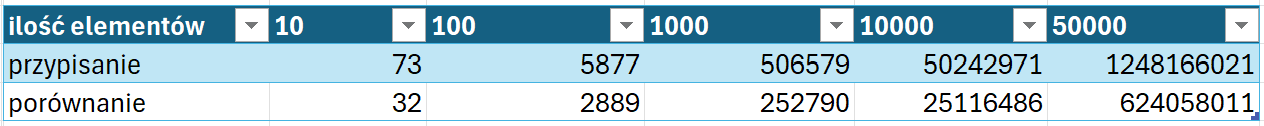
\includegraphics[width=0.9\textwidth]{tabelains1.png}
	\caption{ilość przypisań oraz porównań dla INSERTION SORT}
	\label{fig:tabela1}
\end{figure}


\newpage

\large {Modyfikacja INSERTION SORTA polega na wstawianiu "na raz" dwóch kolejnych elementów tablicy. Zatem duża część kodu działa w dość analogiczny sposób.}



\begin{lstlisting}[language=C++, caption={Fragment 1 funkcji sortującej przez wstawienie z modyfikacją}, numbers=left, frame=single, xleftmargin=20pt, xrightmargin = 1pt]
void INSERTION_SORT_MOD(int A[], int n) {
	for (int s = 1; s < n - 1; s += 2) {
		int pierwszy = A[s];
		int drugi = A[s + 1];
		if (pierwszy > drugi) {
			swap(pierwszy, drugi);
		}
		int k = s - 1;
		while (k >= 0 && A[k] > pierwszy) {
			A[k + 1] = A[k];
			k--;
		}
		A[k + 1] = pierwszy;
		A[k + 2] = drugi;
	}
}

\end{lstlisting}

\large{Pętla zaczyna się od indeksu \(1\) i iteruje z krokiem \(+2\), co pozwala jednocześnie rozpatrywać dwie wartości – \(pierwszy\) i \(drugi\). Następie porównujemy je za pomocą funkcji if i jeśli \(pierwszy\) jest większy zamieniamy miejscami. Funkcja while działa już na tej samej zasadzie co w kodzie bez modyfikacji.}

\newpage

\begin{lstlisting}[language=C++, caption={Fragment 2 funkcji sortującej przez wstawienie z modyfikacją}, numbers=left, frame=single, xleftmargin=20pt, xrightmargin = 1pt]
if (n % 2 == 0) {
	int ostatni = A[n - 1];
	int k = n - 2;
	while (k >= 0 && A[k] > ostatni) {
		A[k + 1] = A[k];
		k--;
	}
	A[k + 1] = ostatni;
}
	
\end{lstlisting}

\large{Przedstawiona modyfikacja jednak wymaga rozważenia przypadku, czy tablica \(A\) ma długość parzystą, czy nieparzystą. Problem pojawia się gdy \(n\) jest parzyste, gdyż ostatni sortowany element nie ma pary (\(ostatni = A[n - 1]\)). Dla \(k\) przypisujemy przedostatni indeks tablicy, które też będzie miejscem rozpoczęcia wstawiania elementu \(ostatni\). Pętla \(while\) działa identycznie jak ta w podstawowym INSERTION SORCIE, z uwagą, że naszym \(key\) jest \(ostatni\).}

	\section{Algorytm sortowania MERGE SORT (przez scalenie)}
	
\begin{lstlisting}[language=C++, caption={Fragment 1 funkcji sortującej przez scalenie bez modyfikacji}, numbers=left, frame=single, xleftmargin=20pt, xrightmargin = 1pt]
void MERGE(int A[], int p, int s, int k) {
	int n1 = s - p + 1;
	int n2 = k - s;
	int L[n1 + 1];
	int P[n2 + 1];
	L[n1] = INT_MAX;
	P[n2] = INT_MAX;
}
\end{lstlisting}

\large{W przypadku MERGE SORTA ważną rolę odgrywa funkcja MERGE, na której na dobrą sprawę zbudowany jest MERGE SORT. MERGE przyjmuje cztery argumenty: \(p\) - początek, \(s\) - środek oraz \(k\) - koniec. Za ich pomocą dzielimy tablicę na dwie części: lewą (\(n1 = s - p + 1\)) oraz prawą (\(n2 = k - s\)). Definiujemy funkcje pomocnicze L i P o pojemności kolejno \(n1 + 1\) oraz \(n2 + 1\). Następnie ustawiamy ostatni element na "napewno większy" od największego elementu tablicy \(A[]\).}

\begin{lstlisting}[language=C++, caption={Fragment 2 funkcji sortującej przez scalenie bez modyfikacji}, numbers=left, frame=single, xleftmargin=20pt, xrightmargin = 1pt]
int i = 0;
int j = 0;
for (int l = p; l <= k; l++) {
	if (L[i] <= P[j]) {
		A[l] = L[i];
		i++;
	} else {
		A[l] = P[j];
		j++;
	}
}
\end{lstlisting}
\large{Po przypisaniu z lewej części do zmiennej \(L\) i z prawej części \(P\) resetujemy wskaźniki \(i\) oraz \(j\) (które wskazują naszą pozycję w kolejno w L i P).
	
Instrukcja \(if (L[i] \leq P[j])\)} sprawdza, czy bieżący element z \(L\) jest mniejszy lub równy bieżącemu elementowi z \(P\). \\
Jeśli tak, to mniejszy element \(L[i]\) jest wstawiany do tablicy \(A[l]\), a wskaźnik \(i\) jest zwiększany o \(1\), by przejść do następnego elementu w \(L\). \\
Jeśli nie, to mniejszy element \(P[j]\) jest kopiowany do \(A[l]\), a wskaźnik \(j\) jest zwiększany o \(1\), by przejść do następnego elementu w \(P\).}
\\

\begin{lstlisting}[language=C++, caption={Fragment 3 funkcji sortującej przez scalenie bez modyfikacji}, numbers=left, frame=single, xleftmargin=20pt, xrightmargin = 1pt]
void MERGE_SORT(int A[], int p, int k) {
	if (p < k) {
		int s = (p + k) / 2;
		MERGE_SORT(A, p, s);
		MERGE_SORT(A, s + 1, k);
		MERGE(A, p, s, k);
	}
}
\end{lstlisting}
\large{Po przeanalizowaniu funkcji MERGE, możemy przejść do funkcji MERGE SORT, która wylicza srodek tablicy i wywołuje kolejno sortowanie z lewej strony, prawej strony po czym scala obie strony.}

\begin{lstlisting}[language=C++, caption={Fragment 1 funkcji sortującej przez scalenie z modyfikacją}, numbers=left, frame=single, xleftmargin=20pt, xrightmargin = 1pt]
void MERGE_MODYFIKOWANY(int A[], int p, int s1, int s2, int k) {
	int n1 = s1 - p + 1;
	int n2 = s2 - s1;
	int n3 = k - s2;
	int L[n1 + 1];
	int S[n2 + 1];
	int P[n3 + 1];
	L[n1] = INT_MAX;
	S[n2] = INT_MAX;
	P[n3] = INT_MAX;
}
\end{lstlisting}
\large{Modyfikacja MERGE SORTA polegała na podzieleniu tablicy na trzy części zamiast dwóch, wiec cały kod opiera się i ma bardzo podobną budowę do podstawowego MERGE SORTA. Zamiast dwóch części tworzymy trzy \(n1 = s1 - p + 1\), \(n2 = s2 - s1\), \(n3 = k - s2\), a jako, że rozdzielamy tablicę. Pozostała reszta MERGA MODYFIKOWANEGO jak i MERGE SORTA MODYFIKOWANEGO przebiega bardzo podobnie.}



\end{document}



